\section{Auswahl und Beschreibung der Messmethode}
\label{chap:auswahl_beschreibung_methode}

Die Idee der hier erstellte Messmethode, ist der CPU über ein Benchmark einen bestimmt Befehlssatz mehrmals durchlaufen zu lassen und die gesamte Leistung des Gerät zu messen. Optimal wäre nur die Leistung des CPU zu messen. Dafür müsste aber der CPU vom Board ausgelötet werden und eine spezielle dafür gebaute Messvorrichtung gebaut werden. Dazu kommt, dass nicht jedes Board oder Chip alle nötigen Datenblätter für die Beschreibung der Pins frei verfügbar sind. Deshalb wird ein Soc eingesetzt und die gesamte Leistung gemessen. SoC sind verfügbar auf kleine Entwickler-Boards, die keine Lüfter, Laufwerke oder andere Verbraucher die  auf Hinsicht der Leistung störende Unregelmässigkeiten aufweisen würden.



\begin{wrapfigure}{r}{0.6\textwidth}
\centering
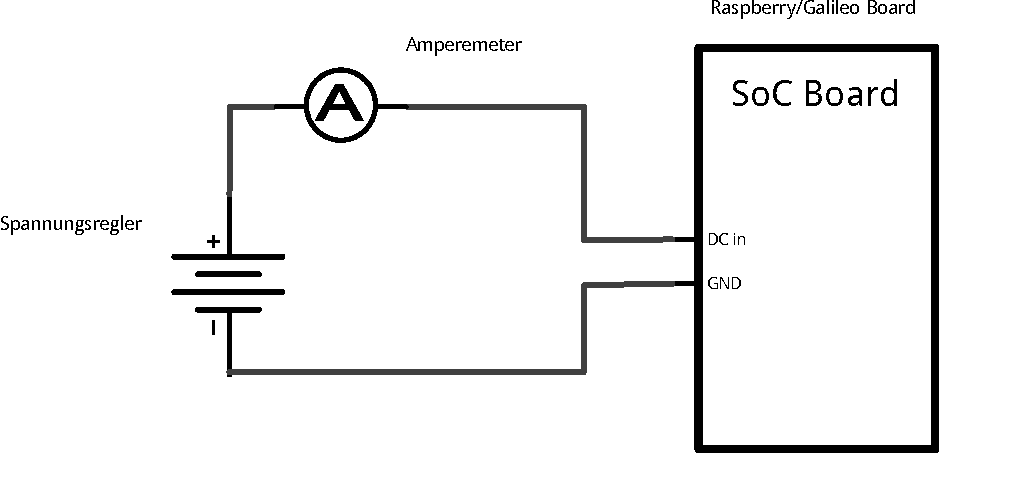
\includegraphics[scale=0.5]{images/schema.pdf}
\caption{Elektroschema für die Messung}
\label{fig:Elektroschema}
\end{wrapfigure}


Die für diese Arbeit verwendete Board werden im nächsten Kapitel beschrieben. Es wird davon Ausgegangen das während Durchführung des Benchmark, die Komponenten auf dem Board abgesehen des CPU, vernachlässigbar kleine Leistungsschwankungen aufweisen. Die Messung erhält somit eine Grundleistung die vom Resultat abgezogen werden muss. Die Speisung erfolgt über ein Spannungsregler der, der Schaltung eine konstante Spannung liefert. Zwischen dem Spannungsregler und der Schaltung ist ein Amperemeter(Multimeter) geschaltet der die Messung vornimmt. In der Abbildung \ref{fig:Elektroschema} ist das Elektroschema und die Platzierung des Amperemeter ersichtlich.
\par
Der eigentliche Kern des Benchmark besteht aus gezielten und kurzen Assembler-Zeilen. Der Assemblercode bewirkt eine Schleife über einen zu testenden Befehlssatz. Damit das Ergebnis über einen längeren Zeitraum gemessen werden kann, wird die Schleife um eine Grössenordnung von 100 Millionen nacheinander wiederholt. Dies erstellt ein Zeitraum für die Messung von ca. einer halbe Minute, auf einem 800MHz CISC-Prozessor.
\par
Während dem durchlaufen des Benchmark darf die Ausführung nicht gestört werden. Jedes moderne Betriebssystem ist Multitasking. Multitasking heisst, dass das Betriebssystem eine Zeitscheibe besitzt und die Ressourcen des CPU abwechslungsweise an die Prozesse verteilt werden. Ein Benchmark darf also nicht gewöhnlicher Prozess von einem Betriebssystem gestartet werden. Würde man das tun hätte man keine Kontrolle wann und wie viel Ressourcen der Benchmark schlussendlich zugesprochen bekommen hätte und dies würde das Messresultat verfälschen. Im Rahmen dieser Arbeit musste eine Methode erarbeitet werden, damit der Benchmark während der Durchführung die volle Ressourcen des CPU bekommt und einen kontrollierten Ablauf garantiert ist.
\par
Die Ursprungsidee was direkt auf Baremetal zu arbeiten. Baremetal ist eine Ausdrucksweise dafür, um direkt auf Hardware zu arbeiten. Bei dieser Methode wird auf das Betriebssystem verzichtet. Nach dem Bootprozess der Hardware wird direkt ein Programm gestartet und ausgeführt. An dieser stelle käme der Benchmark zum Zug. Eine speziell dafür präparierte Portion mit dem Banchmark, würde die Hardware booten und der Benchmark ausführen.
\par
Für die Baremetal-Methode wurde ein funktionstüchtigen Prototyp erstellt. Es zeigten sich aber einigen Nachteile aus. Auf komplexere Hardware mit x86-Prozessoren, ist der Boot-Vorgang um ein vielfaches aufwändiger\cite{intel_boot_process}. Diese Prozessoren-Typen können nicht einfach beim einschalten ein Programmcode ausführen, es müssen vorher eine lange Reihe von Abläufen in der Preboot Phase berücksichtigt und ausgeführt werden. Als zweiter Nachteil der Baremetal-Methode ist die Überprüfung des Benchmark. Um sicher zustellen das der Benchmark Erwartungsgemäss funktioniert oder überhaupt die Feststellung das er ausgeführt wird, benötigt eine Feedback nach aussen. Eine LED würde für dieses Feedback bereits ausreichen. Die GPIO die nötig sind um das LED zu steuern, sind je nach SoC sehr schwierig anzusprechen weil sie über ein PCI-Bus verbunden sind. Das Betriebssystem stellt normalerweise die nötigen Liberies zur Verfügung, um die Komponente wie die GPIO über ein PCI-Bus anzusteuern. Der dritte Nachteil auf eine Methode, ohne Betriebssystem zu arbeiten, ist die aufwändige Vorbereitung jeden einzelnen Test. Für jeden Test muss eine Partition mit dem Benchmark erstellt und auf ein Medium kopiert werden. Die Hardware muss neu gestartet werden
damit die Messung erfolgen kann. Unter den Umständen wird ein automatisierter Betrieb erheblich erschwert.
\par
Aus den oben ernannten Nachteile, wurde ein neues Konzept ausgearbeitet. Das neue Konzept arbeitet auf Linux und bring dadurch bereits alle Vorteile die ein Betriebssystem mit sich bringt. Es muss sicher gestellt werden das der Benchmark ohne Unterbrüche und abgeschirmt von andere Prozesse durchgeführt werden kann. Um dies zu erreichen, wird der Benchmark anstelle des Benutzermodus (engl. User Space) im Kernelmodus (engl. Kernel Space) ausgeführt\cite{Mandl2010}. Ein Programm der innerhalb des Kernelmodus ausgeführt wird muss als Kernelmodul kompiliert und angemeldet werden. Schlussendlich kann nur ein Interrupt das Programm starten. Die genau Beschreibung ist im \autoref{chap:benchmark_basis_interrupts} ausgeführt. Durch die Ausführung des Benchmark werden alle Prozesse die auf dem Betriebssystem parallel ausgeführt werden gestoppt und der Benchmark bekommt die vollen CPU-Ressourcen zugesprochen. In einem Kernelmodul können unterschiedlich Benchmarks gleichzeitig rein kompiliert werden. Somit wird die Ausführung unterschiedliche Test vereinfacht, sowie auch die Automatisierung.

 



 
